\documentclass{article}
\usepackage[ampersand]{easylist}
\usepackage[margin=3.5cm]{geometry}
\usepackage{amsmath}
\usepackage{graphicx}
\usepackage{color}
\usepackage{listings}
\usepackage{parskip}
\usepackage{xcolor}

% We will all remember this as the point where the document prelude went to shit
\definecolor{darkgray}{gray}{0.3}

\PassOptionsToPackage{hyphens}{url}\usepackage[pdftex,
    colorlinks=true,
    linkcolor=darkgray,
    urlcolor=black,
    ]{hyperref}

% Set font to something a bit neater.
%\usepackage{times}
%\renewcommand{\familydefault}{\sfdefault}

\title{%
Brainstorm\\
\large Visualizing brain DTI data using particle systems}

\author{Vegard Itland --- Robin Grundvåg --- Stian Soltvedt}
\date{2018--12--14}

% Helps with overfull hboxes
\emergencystretch3em%
\hfuzz.5pt

% blatantly stolen from the INF226 thing
\definecolor{codebd}{RGB}{226,228,230}
\definecolor{codebg}{RGB}{246,248,250}
\definecolor{codefg}{RGB}{36,41,46}
\newcommand{\code}[1]{\fcolorbox{codebd}{codebg}{\lstinline[basicstyle=\ttfamily\color{codefg}]{#1}}}

\newcommand{\reference}[1]{[\hyperref[ref:#1]{\textbf{#1}}]}
\newcommand{\secref}[2]{\hyperref[sec:#1]{\textbf{#2}}}

\begin{document}
\maketitle
\pagenumbering{arabic}
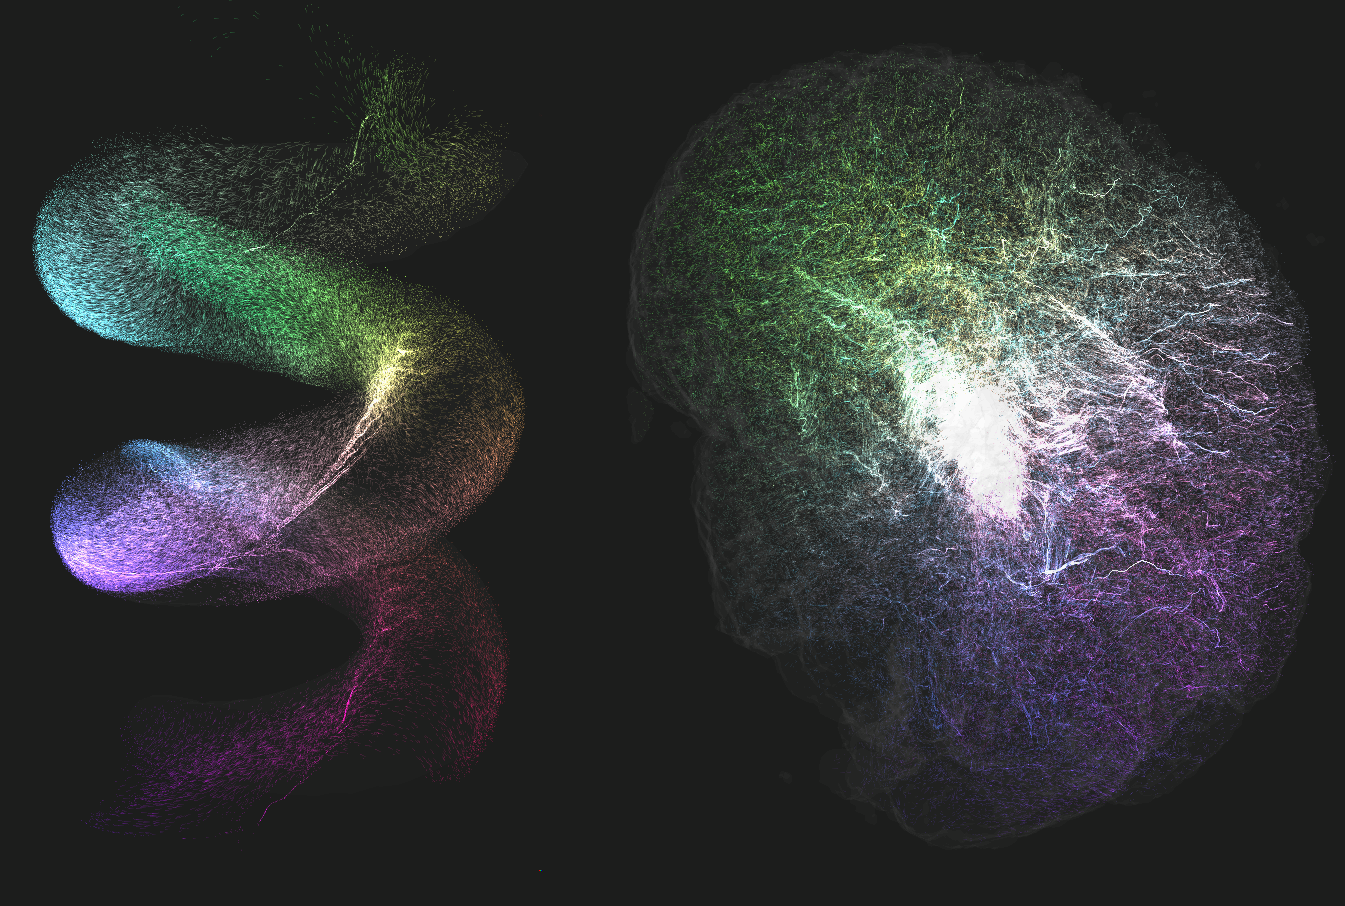
\includegraphics[width=\textwidth]{brainstorm.png}
\section*{Introduction}

Brainstorm is an application attempting to visualize brain diffusion tensor imaging (DTI) data using particle fields. While particle visualization has been used in other contexts such as blood streams, visualization of brain DTI data using particles does not appear to have been attempted, and streamlines are the prevalent visualization method for such datasets.

The application is made to be data-agnostic, meaning that it can read any (compatible format) dataset and visualize it using particles, and is not limited to visualizing brain data.

% NOTE: I felt like the smaller headline was more befitting of an as-such smaller section, but idk
\subsubsection*{DTI data}

Diffusion tensor imaging (DTI) is a medical imaging technique used to measure the interconnectivity of different parts of the brain. The actual measurements are of the direction of possible movement of water molecules in the brain, which in the brain's neural pathways are aligned with the direction of the path. Based on at least six measurements at a given point, we can obtain a tensor representing the vector field's directionality at that point by performing eigenanalysis on the measurement matrix. This enables us to construct a vector field using the measurement data.

\subsection*{Technology}

Brainstorm is written using Rust. Rust was chosen due to our need for a low-level language to easily work with OpenGL directly while also wanting to try something new, as well as part of our team being uncomfortable with C/C++'s manual memory management and pointer arithmetic. This has the benefit of easily compiling to WebAssembly, which opened up the ability to also deploy Brainstorm to a website, without compromising on performance for the desktop version. Unfortunately, this was not as simple as imagined, but despite the extra work required we got it working as we wanted to.

\section*{Implementation}

\subsection*{Making a cross-platform application}

As our group worked on different platforms, we had to settle on a cross-platform language and technology stack. Once we saw the opportunity to also make our application work on the web, we decided to also include web browsers as one of our target platforms. This turned out to be more work than we anticipated.

\subsubsection*{Compiling to all platforms}

Rust compiles to all targets that LLVM can compile to, meaning we have broad platform support on a language level. This includes WebAssembly, although WebAssembly currently has many limitations. These include no threading support, no DOM access, and only being able to pass primitive types and pointers to JavaScript. There's also no API for basic functionality like accessing the date and time.

To get around this, we used the \code{stdweb} \reference{std} library. \code{stdweb} sets up the webpage and handles all calls between JavaScript and Rust automatically so we don't have to manually create external interfaces and callbacks. We also used the \code{cargo-web} \reference{car} tool to automate building the project as a website as well as running the project on a local web-server for testing.

The next obstacle for cross-platform support is rendering and GUI\@. Rust GUI libraries are few and immature, and our needs were very specific as we need direct access to OpenGL to use our shaders. But as far as we could tell, there are no GUI libraries at all that runs on both OpenGL and WebGL\@. That left us to implement our own basic GUI toolkit from scratch.

In order to render the same thing on all targets, we needed was to create a layer of abstraction between our program and OpenGL/WebGL, so that the two API's would not require different code anywhere else in our codebase. Fortunately, we were not the first to attempt this. \code{Kiss3D} \reference{Kis} is a simple 3D graphics engine written in Rust, that we heavily borrowed from when creating our abstraction layer. This made OpenGL and WebGL calls identical and chosen at compile-time, meaning we didn't have to worry about much (although there were still implementation differences, which we will come back to).

\subsubsection*{Writing a GUI toolkit from scratch}

With the GL calls in place, we can start creating data structures that handles drawing primitive triangles to the screen, as well as texturing them. Buttons and sliders can easily be represented, although text labels was a difficult problem. In order to render text, a font must be loaded and parsed, the correct glyphs must be chosen, laid out and rasterized with sub-pixel positioning, and cached on the GPU\@. Fortunately, the \code{RustType} \reference{Rus} library handled most this for us.

Next we made a UI system to do centralized initialization, rendering and event handling for all UI elements. In order to make the UI elements interact with the rest of the application, we created a \code{State} struct that holds all the settings we anticipate to change and pass around a reference to it to the various subsystems, such as the GUI and particle engines. Each UI element can then be loaded with a function that takes a mutable reference to the \code{State} struct and changes it as pre-programmed.

\subsubsection*{Handling files}

Letting the user pick files is a difficult problem on desktop platform --- and we have to support web browsers to boot! Fortunately, the \code{nfd} \reference{nfd} crate provided us with bindings to the C library \code{Native File Dialog} \reference{Nat}, which abstracts away the difference between the native file picker API's on the three main desktop platforms --- Windows, Linux and Mac OS X.

The web required a completely different approach however. Using \code{stdweb} for bindings, we created a small API in JavaScript that provided several functions:

\begin{easylist}
    & Open the file picker and continue.
    & Polling to see if a file has been picked.
    & Get the path of the last picked file.
\end{easylist}

With this API we can retrieve the Base64-encoded file chosen by the user as soon as the browser is finished loading it. After that we decode it to a regular byte stream and can use it as if it was loaded from disk.

\subsection*{Data format}

% TODO: segway from the previous section by bringing up data agnosticism or whatever

This project utilizes the dataset of Gordon Kindlmann's brain \reference{Dif}. The dataset is in the NRRD data format, consisting of a header which provides information about the way the data is structured, and a body which provides the actual data. NRRD is a flexible data format, but our program currently only supports a subset of it which conforms closely to the format described in \reference{Dif}.

The choice of this data format was two-fold: First, this data format is relatively simple to work with from a programming perspective, due to the possibility of separating the header from the data body, the fields which are easy both for humans and computers to parse, and also because the data is arranged in a very simple structure --- just a 3D grid of voxels. Secondly, one of the most easily accessible, open, well-documented brain DTI datasets was in this format. As a bonus, the same page offered a generated helix sample dataset in the same format, which allowed us to test that the method we used was general and would work with other datasets than just the brain.

To be able to translate this data into a format directly understandable by our program, we made a preprocessor which accepts compatible NRRD data and parameters, and spits out the data as a serialized byte array which can be deserialized and used directly by our program. This enables us to store preprocessed data in a file for rapid loading, while also allowing the program to load NRRD data on the fly. Furthermore, it enables an easy way to extend the data in the preprocessing stage through further analysis or, in principle, even manual inspection by experts before loading it into the program, which may be fitted with the capability of interpreting the extensions of this data. An example of this is described in the \secref{prepro}{Pre-processing data analysis} section.

The data body consists of an array of 32 bit floating point values in raw data (big-endian in Kindlmann's brain), which are uniformly spaced measurements arrayed in memory in a 2D-slice-by-slice manner. The data adopts the convention that the Z axis orders the slices in bottom-up fashion, meaning that higher Z memory indices indicate a higher spatial position of the slice. The coordinate (X, Y, Z) in the data thus refers to the measurement in the Yth row and Xth column in the Zth slice of the data from the bottom. The spatial configuration of our particle engine assumed that the X and Y coordinates (in the initial rotation) followed the conventional coordinate space used by computers screens, while Z indicated depth into the screen. This discrepancy was solved by rearranging the structure of the data in the preprocessing stage in order to allow the program to read it the way it expected to.

Each voxel in the dataset consists of a 7-dimensional vector of this format: (Confidence, Dxx, Dxy, Dxz, Dyy, Dyz, Dzz), where:
\begin{easylist}[itemize]
& Confidence is a value representing our confidence that the measurement is signal vs.\@ noise. Usually this value would be binary (zero or one), but it's possible to assign it with continuous values. For instance, a vector with confidence 0.5 would have a 50\% probability of being noise. However, the way we interpret the data, any confidence level lower than 1 is ignored, so it's essentially a mask of the brain.
& The other values form a matrix in this manner:
\end{easylist}

% Must be outside easylist for easylist not to go crazy
% hspace for indent
\hspace{1cm}
\(\begin{bmatrix}
    Dxx & Dxy & Dxz \\
    Dxy & Dyy & Dyz \\
    Dxz & Dyz & Dzz \\
\end{bmatrix}\)

Performing eigenanalysis on this matrix gives us the eigenvectors and the corresponding eigenvalues. We used the Rust crate \code{nalgebra} \reference{Lin} to do this. Finally, we select the most significant eigenvector (using the eigenvalues), calculate the FA value (fractional anisotropy, a scalar indicating how `strongly directional' the data is at that particular point) using the eigenvalues, and push the \((x, y, z, fa)\) vector into our own 3D array in the order our program expects, where \((x, y, z)\) are the \(x\), \(y\) and \(z\) components of the principal eigenvector and \(fa\) is the FA value.

\subsubsection*{Pre-processing data analysis}\label{sec:prepro}

As an enhancement of the data, we attempted to analyze it in order to determine interesting areas from which to perform seeding of particles. We decided that an interesting seeding point would be a point from which particles will travel far, in order to generate long paths. Furthermore, we wanted these points to be somewhat spread out in order to avoid a situation where only starting points in a single area were selected due to that area producing particularly long paths. Thus, we determined that a good strategy would be to attempt to maximize streamline length and spread of starting points.

We ended up settling on an algorithm which uniformly samples points in the dataset and attempts to simulate the particle's path starting from that point using a fixed number of iterations (\(n = 1000\) in our implementation). Starting points were calculated greedily based on the Euclidian distance of the end point to the starting point, and any starting point resulting in a path that collided with previously selected paths was discarded. This was done in order to encourage spread among the points we selected, so that we wouldn't select several close points which merged into one stream. We also attempted to give spread some additional weight by adding in a term considering the sum of the distance of the starting point to all previously selected points.

The final function we attempted to maximize was \(\textrm{dist}(p_e^i, p_s^i) + \textrm{dist}(p_e^i, p_s^i)\cdot{(\sum_{j=1}^{i-1}{\textrm{dist}(p_s^i, p_s^j)})}^{\sqrt{i}}\), where \(p_s^i\) and \(p_e^i\) indicates the start and end point of the \(i\)th selected seeding point, respectively. This function gives the properties:

\begin{easylist}[itemize]
& The initial point is selected only in terms of the distance the particle travels from the starting position, since there are no previous selected points (the second term is zero)
& The sum of the distance between points becomes increasingly important for later seeding points, which helps increase the spread of the points
\end{easylist}

These values were obtained experimentally, and may not be appropriate for all datasets.

Finally, in order to reduce the time it would take to process datasets, we parameterized some options allowing us to sacrifice resolution for speed:

\begin{easylist}[itemize]
& The number of seeding points to calculate
& Step size of uniform sampling (assumption: spatially close values are likely to be similar, so we may be able to skip every other or every third coordinate across each axis and still obtain a reasonably close approximation for a speedup by a factor of \(\textrm{stepsize}^3\))
& Threshold of product of FA values surrounding the point (assumption: interesting seeding locations will be strongly directional, so if the FA value of a point and its neighbors is low, we can ignore it, allowing us to reduce the number of streamlines we have to calculate)
\end{easylist}

Furthermore, the following optimizations were added, possibly sacrificing complete accuracy for speed

\begin{easylist}[itemize]
& We used a nearest neighbor interpolation scheme to avoid having to do trilinear interpolation for every step\footnote{A recently discovered bug reveals that in fact, truncation was used instead of rounding (as nearest neighbor would do), but the result is presumed to be close enough for datasets of reasonably high resolution}
& If the particle's path reached a point where the FA value was zero, it would immediately disqualify the starting point path and move on, assuming that this particle would be destroyed when reaching this point while the program runs
\end{easylist}

\subsubsection*{Output: Custom data format}

The data structure produced by the parser library is as follows:

\begin{verbatim}
#[derive(Serialize, Deserialize)]
struct VectorField {
    width: usize,
    depth: usize,
    height: usize,
    field: Vec<Vec<Vec<(f32,f32,f32,f32)>>>,
    seeding_pts: Vec<(f32,f32,f32)>
}
\end{verbatim}

Using the Rust crate \code{serde} \reference{Ser}, we can serialize this structure as a byte array (using the bincode format \reference{Bin}), and deserialize it for use in the application. The actual internal representation of the vector field in the application itself is flattened due to perceived performance benefits.

\subsection*{OpenGL and WebGL}

Making a renderer work on both the desktop and the web turned out to be trickier than we thought. WebGL's feature set is essentially a subset of OpenGL, with some subtle differences on top. These differences often took significant time and effort to track down and handle properly, but once we got the framework figured out writing the actual algorithms was pretty simple.

Note: From this point forward will I just refer to OpenGL when speaking about our OpenGL / WebGL binding framework.

\subsubsection*{CPU and GPU based particle rendering}

% NOTE: this is a pretty simplistic summary and doesn't account for lifetimes, high-pass filtering, low-pass filtering, etc.
The CPU based particle renderer was our first attempt at drawing particles. It simply keeps a list of particles in memory, that is updated and drawn once per frame. For each particle, it's next position is found by performing a trilinear interpolation on the vector field based on the current particle position. After all particles are updated and moved, they're sent to OpenGL to be drawn as points. Then each point is expanded to a quad by changing the point size to reflect the actual particle size. Then the particle is rounded to a circle instead of a square with a simple fragment shader checking the radius of the fragment from the center of the quad.

While the CPU based approach works well, it could not support as many particles as we wanted. The approach would also make streamlets (fading trails behind the particles) difficult to implement, and would further reduce the number of particles on-screen. One approach to increase it would be to add multi-threading, but this would not work on the web due to WebAssembly limitations. We therefore decided to try a GPU based approach.

% NOTE: Again, this is a simplified summary and does not account for any implementation details of the actual shaders used...
The GPU based particle rendering ended up being a lot harder to implement than we first anticipated, but we were glad we did it in the end. The way it is  implemented is by having an array of textures, where the length of the array is the same as the length of the streamlets. Each texture would then represent the state of the particle system at a given frame, and each pixel would represent the position of a single particle. In order to update the positions, we do the following:

\begin{easylist}
    & Pick a texture containing the current particle state and a 3D texture representing the vector field as input.
    & For each particle, perform a trilinear interpolation in the 3D vector field texture to find the vector at the point it currently is.
    & Add the vector to the current position and save the new particle position as the color on the output texture.
\end{easylist}

In order to display the streamlets in world space we have to do another render pass. We create another array of vertices that represent the vertices that should actually be drawn on the screen, as well as an array of indices based on the streamlets. We then pass these to OpenGL along with the texture array that represents the particle state. We take the positions of the vertices from the colors in the output texture we save earlier and use those as the world space positions. Then we repeat that on the streamlets using the previous world states, based on the gl\_VertexID, and simply place each segment of the streamlet on the earlier calculated position.

Note: This is a simplified version of how it is implemented as WebGL does not support read and write to the same texture, even if it is an array. Due to this are we actually rendering back and forth between two texture arrays, but the logic is mostly the same (just a bit more tedious).

\subsubsection*{Marching Cubes mesh generation}

In order to draw the mesh of the vector field, we implemented the Marching Cubes algorithm. It creates a mesh based on the strength of the vectors in the vector field. This mesh only makes sense when the vector field has edges (like a brain or spiral, rather than noise fields), and we found it very helpful to easily see where in the vector field we were looking. The implementation is not all that special and is very inspired by the linked article by Paul Bourke \reference{Mar}. We simply pass our vector field data and calculate the length of the vectors in order to create a scalar field and use it to construct a mesh.

\section*{Conclusion}

Looking at Brainstorm as it stands right now, it is potentially a useful tool for researchers wanting to visualize DTI scans in a new way. It combines an overview of the overall structure of the field as well as let the user explore the field, guided by the map sliders and filters. It may also have other applications as a result of it's data agnosticism, although this is complicated by the limited set of data formats it currently supports. Support for more formats can fairly trivially be added however.

We do not have any formal plans for future development of Brainstorm, but we have some ideas for tweaks and refactoring that we would like to perform before sharing the project on a bigger stage. Some ideas we have been toying with:

\begin{easylist}
    & Selecting between different interpolation schemes.
    & Additional sliders for particle counts, transparency, etc.
    & Data generation to play with different random vector fields.
    & Improving the high- and low-pass filters to "obstruct" particles physically rather than destroying and respawning them.
        && Likely a difficult task, but would likely significantly improve the visibility of nerve structures in the brain DTI scans.
    & Visualizing probabilistic paths by deviating particle trajectory randomly based on the certainty of the data.
        && Also a time-consuming task, but would leverage a strength of visualizing using particle fields rather than streamlines.
\end{easylist}

\section*{References}

\textbf{[Dif]}\label{ref:Dif}
Diffusion tensor MRI datasets. \url{http://www.sci.utah.edu/~gk/DTI-data/}. (Accessed on 2018--12--14). Brain dataset courtesy of Gordon Kindlmann at the Scientific Computing and Imaging Institute, University of Utah, and Andrew Alexander, W. M. Keck Laboratory for Functional Brain Imaging and Behavior, University of Wisconsin-Madison.

\textbf{[std]}\label{ref:std}
A standard library for the client-side Web. \url{https://github.com/koute/stdweb}. (Accessed on 2018--12--17).

\textbf{[car]}\label{ref:car}
A cargo subcommand for the client-side Web. \url{https://github.com/koute/cargo-web}. (Accessed on 2018--12--17).

\textbf{[Kis]}\label{ref:Kis}
Kiss3D. \url{http://kiss3d.org/}. (Accessed on 2018--12--17).

\textbf{[Rus]}\label{ref:Rus}
RustType. \url{https://github.com/redox-os/rusttype}. (Accessed on 2018--12--17).

\textbf{[nfd]}\label{ref:nfd}
nfd-rs. \url{https://github.com/saurvs/nfd-rs}. (Accessed on 2018--12--17).

\textbf{[Nat]}\label{ref:Nat}
Native File Dialog. \url{https://github.com/mlabbe/nativefiledialog} (Accessed on 2018--12--17).

\textbf{[Lin]}\label{ref:Lin}
Linear algebra library. \url{https://www.nalgebra.org/}. (Accessed on 2018--12--17).

\textbf{[Ser]}\label{ref:Ser}
Serde. \url{https://serde.rs/}. (Accessed on 2018--12--17).

\textbf{[Bin]}\label{ref:Bin}
Bincode. \url{https://github.com/TyOverby/bincode}. (Accessed on 2018--12--17).

\textbf{[Mar]}\label{ref:Mar}
Polygonising a scalar field (Marching Cubes). \url{http://paulbourke.net/geometry/polygonise/}. (Accessed on 2018--12--16)

\end{document}
